\section{Analysis}
\subsection{The Conductor Loops}
To calculate the $B_z$ value and the dipole moment $p$, there are two different way. The first one is to calculate the theoretical magnetic field as well as dipole moment by using the properties of the conductor loop and the applied voltage.\par
Here the equation \ref{Dipolmoment1} was used.
\begin{equation}
	p(R)=AI(R)=\pi r^2I(R)=\pi r^2 \frac{U}{R}
	\label{Dipolmoment1}
\end{equation}
The error is than computed using Gaussian error propagation by following equation:
\begin{equation}
	\sigma_p=\sqrt{\left(\frac{\pi U r \sigma_r}{R}\right)^2+\left(\frac{\pi r^2 \sigma_U}{R}\right)^2+\left(\frac{\pi r^2 U \sigma_R}{R^2}\right)^2}
\end{equation}
The diameter $d$ of the loop was measured multiples times and the mean was taken to get the radius . The error of the mean was calculated using equation \ref{Meanerror}. After this the value was divided by $2$ to get the radius.\par
\begin{equation}
	\sigma_x=\sqrt{\left(\frac{1}{n-1}\sum_{i=1}^{n}(x_i-\bar{x})^2\right)}
	\label{Meanerror}
\end{equation}
The voltage was gained by measuring the two attached batteries and adding them together. The values for the different resistors were given in the manual of the experiment\cite{anleitung} and are noted in table \ref{tableResi}.\par  
\begin{equation*}
	r = (1.558 \pm 0.010)\,mm
\end{equation*}
\begin{equation*}
	U_{ges} = U_1 + U_2 = (1.459\pm0.005 + 1.494\pm0.005)\,\text{V} = (2.9530\pm0.0007)\,\text{V}
\end{equation*}
\begin{table}[ht]
	\begin{Dtabular}[1.1]{|c|c|c|c|c|c|}
		\hline
		&Resistor 1&Resistor 2&Resistor 3&Resistor 4&Resistor 5\\
		\hline
		$\Omega$&$51.47\pm0.05$&$100.80\pm0.10$&$300.80\pm0.30$&$510.6\pm0.5$&$1000.0\pm1.0$\\
		\hline
	\end{Dtabular}
	\centering
	\caption[Resistors]{Different Resistors for the five conductor loop measurements.}
	\label{tableResi}
\end{table}
With this the dipole moment for the different Resistors was calculated and are written down in table \ref{Messwerte1}.\par
It can now be used to compute the magnetic field $B_z$ using equation \ref{DipolFeld}.
\begin{equation}
	B_z = \frac{\mu_0 p}{2\pi z^3}
	\label{DipolFeld}
\end{equation}
In this equation the value z is the distance of the probe to the SQUID. This was measured by measuring the length of the kryostat from top to the probe as well as from the top to the SQUID. The difference of both is the distance from probe to SQUID. To decrease the errors the mean of multiple distance measurements were taken.
\begin{equation*}
	z=(2.65 \pm 0.12)\,\text{cm}
\end{equation*}
The with that calculated value $B_z$ is also in table \ref{Messwerte1}.
\begin{table}[ht]
	\begin{Dtabular}[1.1]{|c|c|c|}
		\hline
		&$p$\,[Am$^2$]&$B_z$\,[T]\\
		\hline
		R1&$\left(8.75 \pm 0.11\right) \times 10^{-7} $&$\left(9.4 \pm 1.2\right) \times 10^{-9}$\\
		\hline
		R2&$\left(4.47 \pm 0.06\right) \times 10^{-7} $&$\left(4.8 \pm 0.6\right) \times 10^{-9}$\\
		\hline
		R3&$\left(1.498 \pm 0.020\right) \times 10^{-7}$ &$\left(1.61 \pm 0.21\right) \times 10^{-9}$\\
		\hline
		R4&$\left(8.82 \pm 0.12\right) \times 10^{-8} $&$\left(9.5 \pm 1.2\right) \times 10^{-10}$\\
		\hline
		R5&$\left(4.51 \pm 0.06\right) \times 10^{-8}$ &$\left(4.8 \pm 0.6\right) \times 10^{-10}$\\ 
		\hline
		
	\end{Dtabular}
	\centering
	\caption[Values of Dipole Moment and Magnetic Field]{Values of the magnetic field and the dipole moment for the five different resistors. Calculated by using equation \ref{Dipolmoment1} and \ref{DipolFeld}}
	\label{Messwerte1}
\end{table} 
\newpage
The other way to calculate the dipole moment and magnetic field was by using the measured signals of the SQUID. Here the signal shapes were fitted with the help of Pythons package  \verb|scipy.optimize| with the method \verb|curve_fit|. Here the form given in equation \ref{Sinusfit} was used. With that the offset $a$, the frequency $\omega=c$ as well as the amplitude $b=\Delta V$ can be calculated. 
\begin{equation}
	f(x)=a+b\sin(cx+d)
	\label{Sinusfit}
\end{equation}
An example of the fits can be seen in figure \ref{Fit1} the other ones are in the appendix.\par
The parameters $b$ of the different measurements for each resistor were taken and the weighted mean of them was taken. For this mean the equation \ref{WMean} and \ref{Er_WMean} were used. The values are listed in table \ref{Messwerte2}. \par
\begin{equation}
	\bar{x}_g=\frac{\sum_ig_ix_i}{\sum_ig_i} \qquad \text{with} \qquad g_i=\frac{1}{\sigma_i^2}
	\label{WMean}
\end{equation}
\begin{equation}
	\sigma_{\bar{x}_g}=\frac{1}{\sqrt{\sum_i\nicefrac{1}{\sigma_i^2}}}
	\label{Er_WMean}
\end{equation}
With these voltages the magnetic field $B_z$ can be computed using equation \ref{Bz}. An similar to the calculation for the theoretical values equation \ref{DipolFeld} can be used to gain the dipole moment $p$.
\begin{equation}
	B_z=F\frac{\Delta V}{s_i}
	\label{Bz}
\end{equation}
The value of $F$ the field flux coefficient is $9.3\,\frac{\text{nT}}{\Phi_0}$ and $s_i$ is transfer coefficient. This one can be looked up in the manual\cite{anleitung}. For the conductor loops a FB-R resistance of $100$\,k$\Omega$ was chosen which leads to a $s_i$ value of $1900\,\frac{mV}{\Phi_0}$. The values of the calculated magnetic field and dipole moment are noted in table \ref{Messwerte2}
\begin{table}[ht]
	\begin{Dtabular}[1.1]{|c|c|c|c|}
		\hline
		&$p$[Am$^2$]&$B_z$[T]&$\Delta V$\,[V]\\
		\hline
		R1&$\left(2.19 \pm 0.29\right) \times 10^{-7} $&$\left(2.356 \pm 0.007\right) \times 10^{-9} $&$0.2407 \pm 0.0007$\\
		\hline
		R2&$\left(1.18 \pm 0.15\right) \times 10^{-7} $&$\left(1.271 \pm 0.007\right) \times 10^{-9} $&$0.1298 \pm 0.0007$\\
		\hline
		R3&$\left(3.9 \pm 0.5\right) \times 10^{-8} $&$\left(4.17 \pm 0.08\right) \times 10^{-10} $&$0.0426 \pm 0.0008$\\
		\hline
		R4&$\left(2.36 \pm 0.31\right) \times 10^{-8}$&$\left(2.54 \pm 0.05\right) \times 10^{-10}$&$0.0259 \pm 0.0005$\\
		\hline
		R5&$\left(1.37 \pm 0.19\right) \times 10^{-8} $&$\left(1.47 \pm 0.06\right) \times 10^{-10}$&$0.0150 \pm 0.0006$\\
		\hline
	\end{Dtabular}
	\centering
	\caption[Values of the Loops with the Fit Method]{Measured values for the different conductor loops using the fits of the SQUID signals.}
	\label{Messwerte2}
\end{table}
\begin{figure}[ht]
	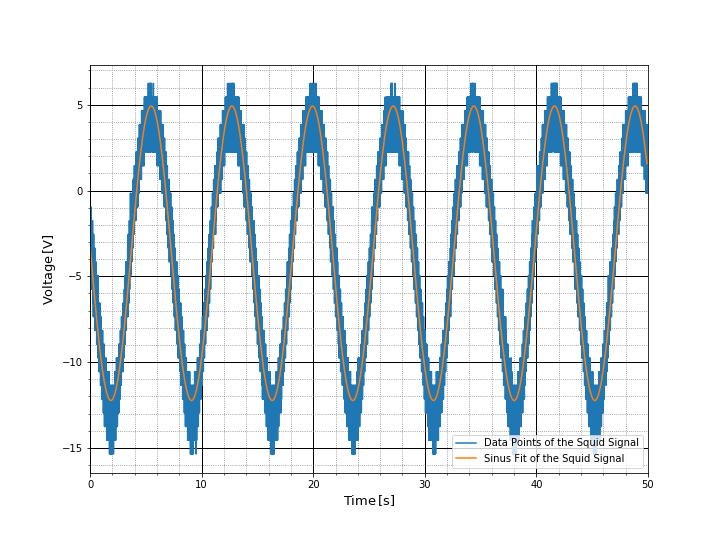
\includegraphics[scale=0.5]{Bild/r1_5_2}
	\centering
	\caption[Example of the Data Plots with SInus Fit]{In blue the signal coming from the SQUID and in orange the sinus fit to the data points.}
\end{figure}
\FloatBarrier
\subsection{Other Samples}
During the measurement other samples were tested with the SQUID. The SQUID signals were analysed in a similar way to the conductor Loops before. The sinus of the form \ref{Sinusfit} was fitted on the signal. The mean of amplitude which is parameter $b$ was computed for the different samples and with this the magnetic field $B_z$ and dipole moment could be calculated and can be found in table \ref{Messwerte3} in the table below.\par
\begin{table}[ht]
	\begin{Dtabular}[1.1]{|c|c|c|c|}
		\hline
		&$p$[Am$^2$]&$B_z$[T]&$\Delta V$\,[V]\\
		\hline
		Iron chips&$\left(1.84 \pm 0.25\right) \times 10^{-8}  $&$\left(1.98 \pm 0.07\right) \times 10^{-10}  $&$0.0202 \pm 0.0007 $\\
		\hline
		Gold lamella&$ \left(3.2 \pm 0.4\right) \times 10^{-8} $&$ \left(3.42 \pm 0.12\right) \times 10^{-10} $&$0.0349 \pm 0.0012 $\\
		\hline
		Magnet chips&$\left(7.8 \pm 1.0\right) \times 10^{-6}  $&$\left(8.408 \pm 0.030\right) \times 10^{-8}  $&$8.589 \pm 0.031 $\\
		\hline
		Stone&$\left(7.4 \pm 1.1\right) \times 10^{-10}  $&$ \left(7.9 \pm 0.5\right) \times 10^{-12} $&$ 0.00081 \pm 0.00005$\\
		\hline
		Magnet&$0.000262 \pm 0.000034 $&$\left(2.814 \pm 0.014\right) \times 10^{-6}  $&$6.355 \pm 0.031 $\\
		\hline
	\end{Dtabular}
	\centering
	\caption[Values of the Samples with the Fit Method]{Measured and calculated values for different materials and forms of samples.}
	\label{Messwerte3}
\end{table}
\subsection{Polar Representation}
For the samples and conductor loops the polar representation should be plotted. For this one period of the data points was taken. With the help of the coordinate transformation of the manual\cite{anleitung}:
\begin{equation}
	x_i=|B_z|\cdot \cos(\alpha)
\end{equation}
\begin{equation}
	y_i=|B_z|\cdot \sin(\alpha)
\end{equation}
Here $\alpha$ is the rotation angle. For the stone the polar representation can be seen in figure \ref{Stone}, the rest is in the appendix.
\begin{figure}[ht]
	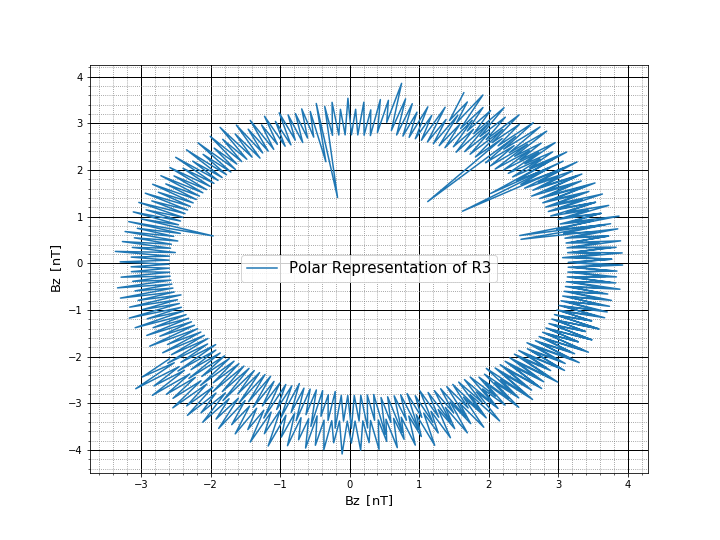
\includegraphics[scale=0.5]{Bild/R3}
	\centering
	\caption[Polar Representation for R2 Conductor Loop]{Polar Representation for one period of the signal coming from the R2 Conductor Loop.}
	\ref{Stone}
\end{figure}\\